\documentclass{standalone}
\usepackage{tikz}
\usetikzlibrary{patterns, positioning}
\usepackage[sfdefault]{ClearSans} %% option 'sfdefault' activates Clear Sans as the default text font
\usepackage[T1]{fontenc}

\begin{document}
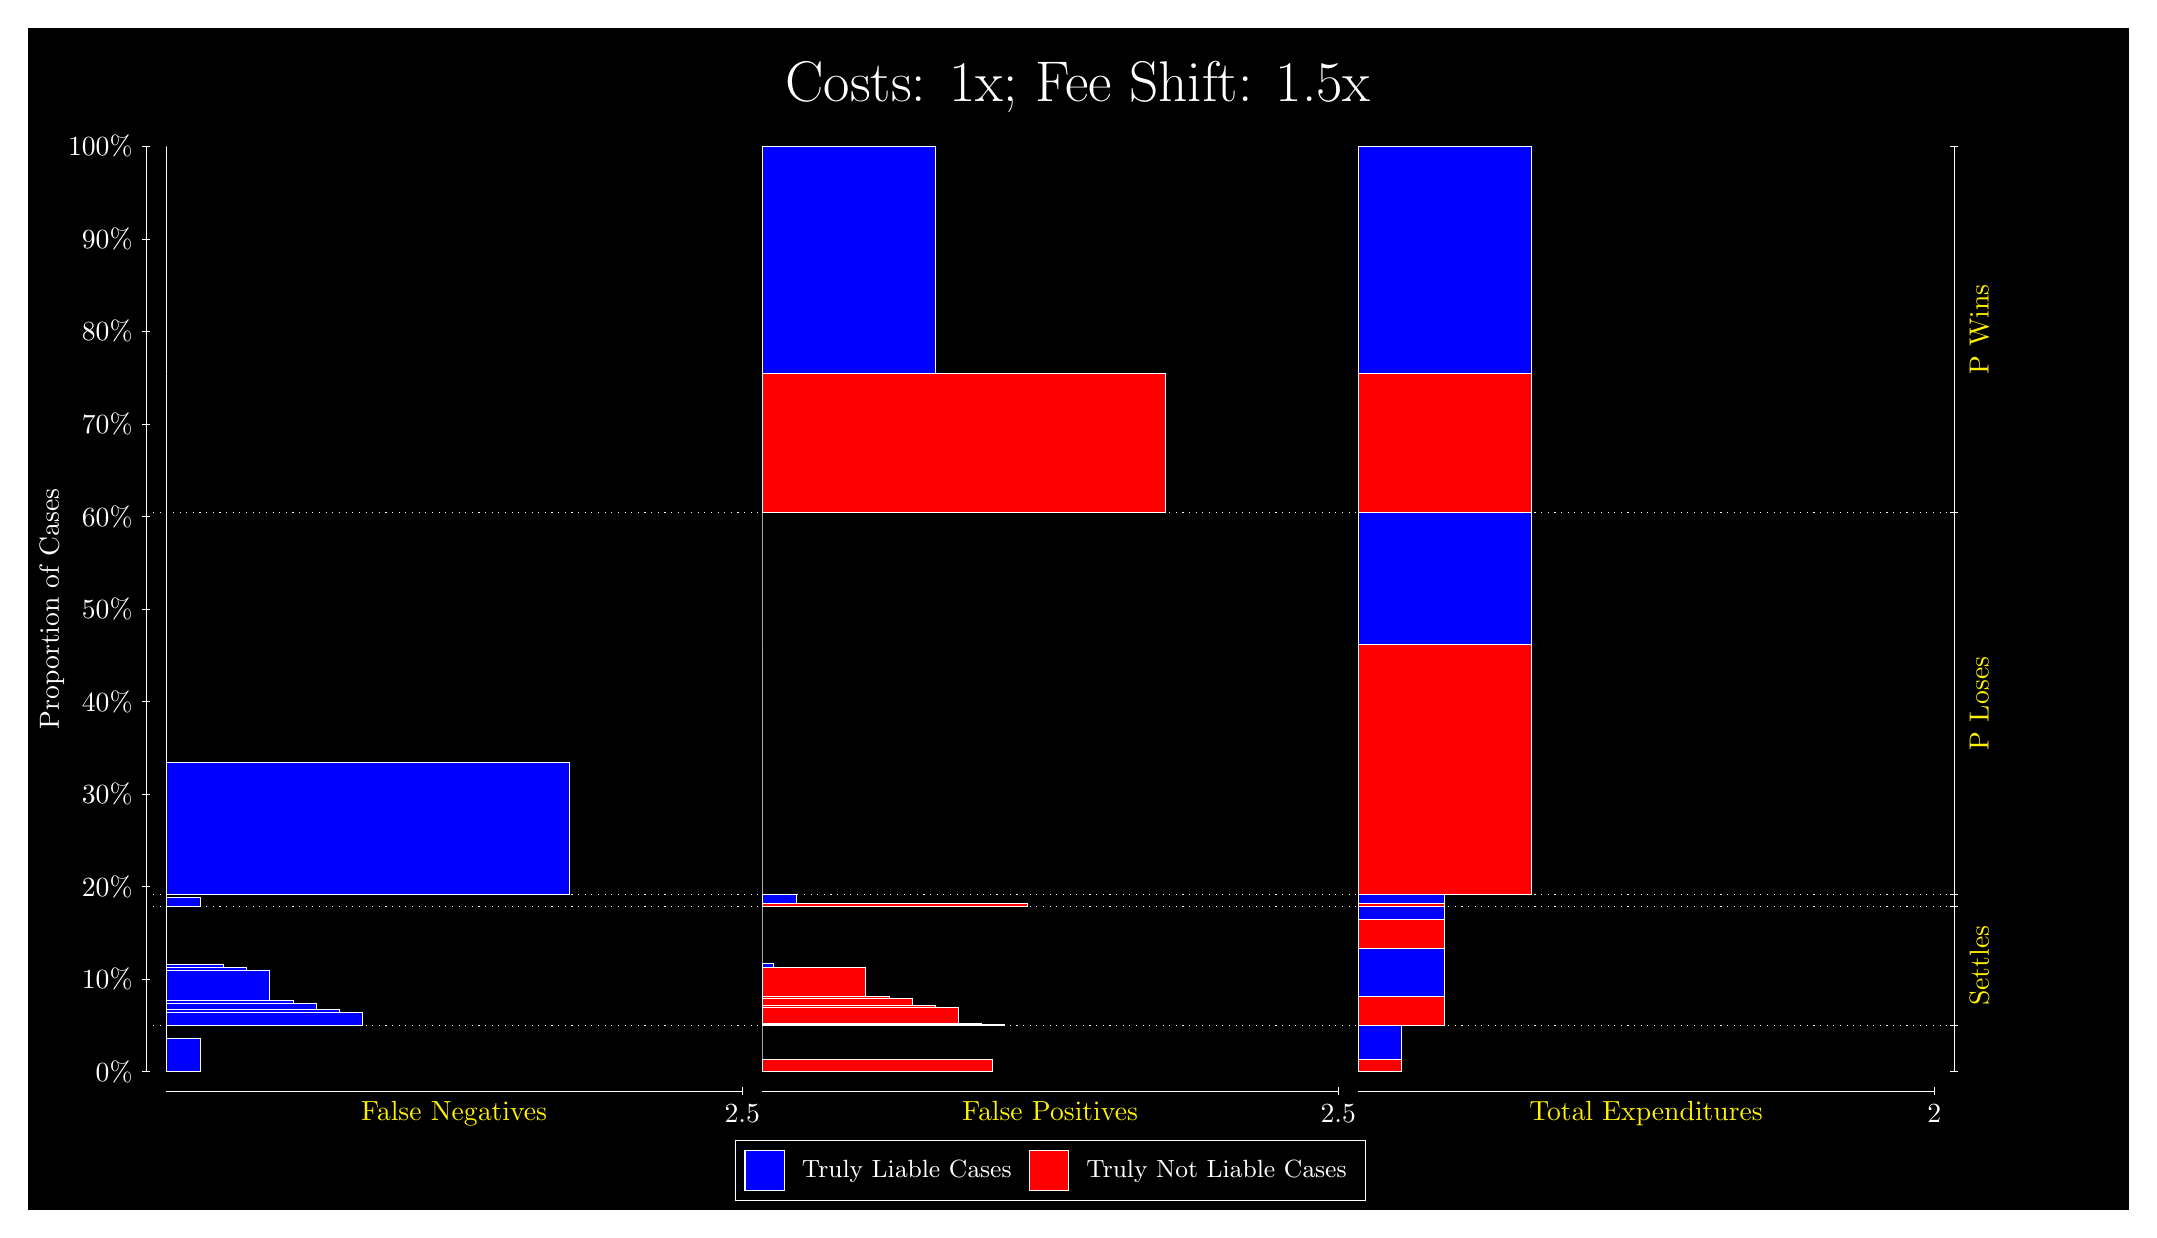
\begin{tikzpicture}
\draw[fill=black] (0,0) rectangle (26.667,15);
\draw[text=white] (0,13.5) rectangle (26.667,15) node[midway] {\huge Costs: 1x; Fee Shift: 1.5x};
\draw[white, very thin] (1.5,1.75) -- (1.5,13.5);
\node[rotate=90, text=white, anchor=center] at (0.3, 7.625) {Proportion of Cases};
\draw[white, very thin] (1.45,1.75) -- (1.55,1.75);
\node[text=white, anchor=east] at (1.45, 1.75) {0\%};
\draw[white, very thin] (1.45,2.925) -- (1.55,2.925);
\node[text=white, anchor=east] at (1.45, 2.925) {10\%};
\draw[white, very thin] (1.45,4.1) -- (1.55,4.1);
\node[text=white, anchor=east] at (1.45, 4.1) {20\%};
\draw[white, very thin] (1.45,5.275) -- (1.55,5.275);
\node[text=white, anchor=east] at (1.45, 5.275) {30\%};
\draw[white, very thin] (1.45,6.45) -- (1.55,6.45);
\node[text=white, anchor=east] at (1.45, 6.45) {40\%};
\draw[white, very thin] (1.45,7.625) -- (1.55,7.625);
\node[text=white, anchor=east] at (1.45, 7.625) {50\%};
\draw[white, very thin] (1.45,8.8) -- (1.55,8.8);
\node[text=white, anchor=east] at (1.45, 8.8) {60\%};
\draw[white, very thin] (1.45,9.975) -- (1.55,9.975);
\node[text=white, anchor=east] at (1.45, 9.975) {70\%};
\draw[white, very thin] (1.45,11.15) -- (1.55,11.15);
\node[text=white, anchor=east] at (1.45, 11.15) {80\%};
\draw[white, very thin] (1.45,12.325) -- (1.55,12.325);
\node[text=white, anchor=east] at (1.45, 12.325) {90\%};
\draw[white, very thin] (1.45,13.5) -- (1.55,13.5);
\node[text=white, anchor=east] at (1.45, 13.5) {100\%};

\draw[white, very thin] (24.457,1.75) -- (24.457,13.5);
\draw[white, very thin] (24.407,1.75) -- (24.507,1.75);
\node[anchor=west] at (24.407, 1.75) {};
\draw[white, very thin] (24.407,2.3383) -- (24.507,2.3383);
\node[anchor=west] at (24.407, 2.3383) {};
\draw[white, very thin] (24.407,3.8507) -- (24.507,3.8507);
\node[anchor=west] at (24.407, 3.8507) {};
\draw[white, very thin] (24.407,4.0026) -- (24.507,4.0026);
\node[anchor=west] at (24.407, 4.0026) {};
\draw[white, very thin] (24.407,8.848) -- (24.507,8.848);
\node[anchor=west] at (24.407, 8.848) {};
\draw[white, very thin] (24.407,13.5) -- (24.507,13.5);
\node[anchor=west] at (24.407, 13.5) {};

\draw[white, very thin, fill=blue] (1.75,1.75) rectangle (2.1891,2.1768);
\draw[white, very thin, fill=red] (1.75,2.1768) rectangle (1.75,2.3383);
\draw[white, very thin, fill=blue] (1.75,2.3383) rectangle (4.2384,2.5073);
\draw[white, very thin, fill=blue] (1.75,2.5073) rectangle (3.9457,2.5367);
\draw[white, very thin, fill=blue] (1.75,2.5367) rectangle (3.6529,2.6223);
\draw[white, very thin, fill=blue] (1.75,2.6223) rectangle (3.3602,2.6536);
\draw[white, very thin, fill=blue] (1.75,2.6536) rectangle (3.0674,3.0325);
\draw[white, very thin, fill=blue] (1.75,3.0325) rectangle (2.7746,3.07);
\draw[white, very thin, fill=blue] (1.75,3.07) rectangle (2.4819,3.1138);
\draw[white, very thin, fill=red] (1.75,3.1138) rectangle (1.75,3.8507);
\draw[white, very thin, fill=blue] (1.75,3.8507) rectangle (2.1891,3.9637);
\draw[white, very thin, fill=red] (1.75,3.9637) rectangle (1.75,4.0026);
\draw[white, very thin, fill=blue] (1.75,4.0026) rectangle (6.8732,5.6794);
\draw[white, very thin, fill=red] (1.75,5.6794) rectangle (1.75,8.848);
\draw[white, very thin, fill=red] (1.75,8.848) rectangle (1.75,10.617);
\draw[white, very thin, fill=blue] (1.75,10.617) rectangle (1.75,13.5);
\draw[white, very thin, fill=red] (9.3189,1.75) rectangle (12.246,1.9115);
\draw[white, very thin, fill=blue] (9.3189,1.9115) rectangle (9.3189,2.3383);
\draw[white, very thin, fill=red] (9.3189,2.3383) rectangle (12.393,2.3512);
\draw[white, very thin, fill=red] (9.3189,2.3512) rectangle (12.1,2.3655);
\draw[white, very thin, fill=red] (9.3189,2.3655) rectangle (11.807,2.5602);
\draw[white, very thin, fill=red] (9.3189,2.5602) rectangle (11.515,2.5901);
\draw[white, very thin, fill=red] (9.3189,2.5901) rectangle (11.222,2.6771);
\draw[white, very thin, fill=red] (9.3189,2.6771) rectangle (10.929,2.7058);
\draw[white, very thin, fill=red] (9.3189,2.7058) rectangle (10.636,3.0752);
\draw[white, very thin, fill=blue] (9.3189,3.0752) rectangle (9.4652,3.119);
\draw[white, very thin, fill=blue] (9.3189,3.119) rectangle (9.3189,3.8507);
\draw[white, very thin, fill=red] (9.3189,3.8507) rectangle (12.686,3.8897);
\draw[white, very thin, fill=blue] (9.3189,3.8897) rectangle (9.758,4.0026);
\draw[white, very thin, fill=red] (9.3189,4.0026) rectangle (9.3189,7.1712);
\draw[white, very thin, fill=blue] (9.3189,7.1712) rectangle (9.3189,8.848);
\draw[white, very thin, fill=red] (9.3189,8.848) rectangle (14.442,10.617);
\draw[white, very thin, fill=blue] (9.3189,10.617) rectangle (11.515,13.5);
\draw[white, very thin, fill=red] (16.888,1.75) rectangle (17.437,1.9115);
\draw[white, very thin, fill=blue] (16.888,1.9115) rectangle (17.437,2.3383);
\draw[white, very thin, fill=red] (16.888,2.3383) rectangle (17.986,2.7058);
\draw[white, very thin, fill=blue] (16.888,2.7058) rectangle (17.986,3.3124);
\draw[white, very thin, fill=red] (16.888,3.3124) rectangle (17.986,3.6817);
\draw[white, very thin, fill=blue] (16.888,3.6817) rectangle (17.986,3.8507);
\draw[white, very thin, fill=red] (16.888,3.8507) rectangle (17.986,3.8897);
\draw[white, very thin, fill=blue] (16.888,3.8897) rectangle (17.986,4.0026);
\draw[white, very thin, fill=red] (16.888,4.0026) rectangle (19.083,7.1712);
\draw[white, very thin, fill=blue] (16.888,7.1712) rectangle (19.083,8.848);
\draw[white, very thin, fill=red] (16.888,8.848) rectangle (19.083,10.617);
\draw[white, very thin, fill=blue] (16.888,10.617) rectangle (19.083,13.5);
\draw[white, dotted] (1.5,2.3383) -- (24.457,2.3383);
\draw[white, dotted] (1.5,3.8507) -- (24.457,3.8507);
\draw[white, dotted] (1.5,4.0026) -- (24.457,4.0026);
\draw[white, dotted] (1.5,8.848) -- (24.457,8.848);
\draw[white, very thin] (1.75,1.5) -- (9.0689,1.5);
\node[text=yellow, anchor=north] at (5.4094, 1.5) {False Negatives};
\draw[white, very thin] (9.0689,1.45) -- (9.0689,1.55);
\node[text=white, anchor=north] at (9.0689, 1.45) {2.5};

\draw[white, very thin] (9.3189,1.5) -- (16.638,1.5);
\node[text=yellow, anchor=north] at (12.978, 1.5) {False Positives};
\draw[white, very thin] (16.638,1.45) -- (16.638,1.55);
\node[text=white, anchor=north] at (16.638, 1.45) {2.5};

\draw[white, very thin] (16.888,1.5) -- (24.207,1.5);
\node[text=yellow, anchor=north] at (20.547, 1.5) {Total Expenditures};
\draw[white, very thin] (24.207,1.45) -- (24.207,1.55);
\node[text=white, anchor=north] at (24.207, 1.45) {2};


\node[text=yellow, centered, rotate=90] at (24.777, 3.0945) {Settles};

\node[text=yellow, centered, rotate=90] at (24.777, 6.4253) {P Loses};
\node[text=yellow, centered, rotate=90] at (24.777, 11.174) {P Wins};

\draw (12.978300999999998,1.5) node[draw=none] (baseCoordinate) {};
\begin{scope}[align=center]
        \matrix[scale=0.5, draw=white, below=0.5cm of baseCoordinate, nodes={draw}, column sep=0.1cm]{
            \node[rectangle, draw, minimum width=0.5cm, minimum height=0.5cm, fill=blue] {}; &
            \node[draw=none, font=\small, text=white] (B) {Truly Liable Cases}; &
            \node[rectangle, draw, minimum width=0.5cm, minimum height=0.5cm, fill=red] {}; &
            \node[draw=none, font=\small, text=white] (B) {Truly Not Liable Cases}; \\
            };
\end{scope}

\end{tikzpicture}
\end{document}